\clearpage

\section{MS Windows IP Tunnel}

\begin{tcolorbox}	
	\begin{tabular}{p{2.75cm} p{0.2cm} p{10.5cm}} 	
		\textbf{Header File}   &:& ms$\_$windows$\_$ip$\_$tunnel$\_*$.h \\
		\textbf{Source File}   &:& ms$\_$windows$\_$ip$\_$tunnel$\_*$.cpp \\
        \textbf{Version}       &:& 20180815 (Jo\~ao Coelho) \\
	\end{tabular}
\end{tcolorbox}

This block works in two ways: one way with one input and zero output signals (as client/sender) and the other one with zero input and one output signal (as server/receiver).
MS Windows IP Tunnel is duplicated onto two machines; the first takes samples out of the input buffer until it's empty and transmits them to the IP Tunnel on the second machine through a TCP/IP connection. The IP Tunnel on the second machine receives the signal and outputs it to the output buffer.
It's only necessary to specify the ip address of the remote machine and its TCP port.
Only works on windows due to the Ws2tcpip.h header and ws2\_32 library and it is compatible and tested with SDK v8.1 and v10.0.18362.0.

\subsection*{Input Parameters}

\begin{table}[h]
	\centering
	\begin{tabular}{|l|c|c|c|p{50mm}|}
		\cline{1-5}
		\textbf{Parameter} & \textbf{Type} & \textbf{Values} &   \textbf{Default}& \textbf{Brief Description} \\ \cline{1-5}
		
        displayNumberOfSamples & bool & true/false & true & If true, number of samples sent and received are displayed.\\ \cline{1-5}
		numberOfTrials & int & any & $10$ & Number of trials after a connection has been refused.\\ \cline{1-5}
		remoteMachineIpAddress & string & any & "127.0.0.1" & IP Address of Remote Machine.\\ \cline{1-5}
		tcpPort & int & any & $54000$ & TCP port used to connect to server.\\ \cline{1-5}
		timeIntervalSeconds & int & any & $3$ & Time interval before trying to connect again after a connection has been refused (seconds).\\ \cline{1-5}
	\end{tabular}
	\caption{MS Windows IP Tunnel input parameters}
	\label{table:ipt_in_par}
\end{table}

%\subsection*{State Variables}
%
%\begin{table}[h]
%	\centering
%	\begin{tabular}{|c|c|p{30mm}|c|ccp{60mm}}
%		\cline{1-4}
%		\textbf{Parameter} & \textbf{Type} & \textbf{Values} &   \textbf{Default}& \\ \cline{1-4}
%		alive & bool & true/false & true \\ \cline{1-4}
%	\end{tabular}
%	\caption{MS Windows IP Tunnel state variables}
%	\label{table:iptunnel_st_var}
%\end{table}

\subsection*{Methods}
%
IPTunnel(vector$<$Signal *$>$ \&InputSig, vector$<$Signal *$>$ \&OutputSig)
\bigbreak
void initialize(void);
\bigbreak
bool runBlock(void);
\bigbreak
void terminate(void);
\bigbreak
void ipTunnelSendInt(int space);
\bigbreak
int ipTunnelRecvInt();
\bigbreak
int ipTunnelPut(T object);
\bigbreak
void setDisplayNumberOfSamples(bool opt);
\bigbreak
bool getDisplayNumberOfSamples();
\bigbreak
bool server();
\bigbreak
bool client();



\subsection*{Functional Description}

The IP Tunnel block transfers signals from one machine to another so it continues the simulation in two different computers. This block is duplicated onto two machines, one with only input (client) and other with only output signals (server). After being executed, the input signal's buffer (1) will be empty and this block will transmit this signal to the other block. The second block will output this signal to the output buffer (4). An architecture "Server - Client" is used to establish a TCP/IP channel between the two blocks (2 and 3). The block without input signal is the server (receiver) and the block with input signal is the client (transmitter). After the connection is established, server sends the "space" of its buffer (maximum signal size that can be received) and client responds with the "process" (signal size that is going to be transmitted) and with an integer representing the type of signal. Subsequently, the transmission of the signal starts and the simulation continues normally on both machines.

\begin{figure}[h]
	\centering
	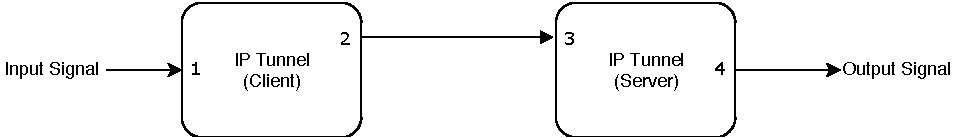
\includegraphics[width=1.0\textwidth]{./lib/ms_windows_ip_tunnel/figures/StructureTCPIP4.pdf}
	\label{IP Tunnel Block}\caption{MS Windows IP Tunnel block}
\end{figure}